\documentclass[12pt,a4paper]{report}

\usepackage[utf8]{inputenc}
\usepackage[T1]{fontenc}
\usepackage[spanish,es-tabla]{babel}
\usepackage{../lab-doc}


\doctitulo{Manual de Usuario del Laboratorio de Archivística y Humanidades Digitales}
\docbanner{Manual de Usuario}
\docsubtitulo{Manual de usuario}
\docautores{Equipo del Laboratorio de Archivística\\Hexoneira:\\ Juan Carlos Quintero y\\ Nicolas Acevedo\\ Universidad Distrital Francisco José de Caldas}
\docciudad{Bogotá, Colombia}
\docfecha{2026}

\begin{document}

\portadalab

\tableofcontents
\thispagestyle{chapternoline}

\chapter{Introducción}

El \textbf{Laboratorio de Archivística y Humanidades Digitales} es un espacio
académico de la Universidad Distrital Francisco José de Caldas dedicado a la
gestión, análisis y transformación de la información mediante tecnologías
digitales. El laboratorio integra herramientas de código abierto y equipos
especializados para apoyar la investigación, la docencia y la extensión en
materia archivística.

Este manual describe, paso a paso, el uso del \textbf{portal web del
laboratorio}: cómo acceder a él, cómo navegar por sus secciones, cómo solicitar
equipos y salas, y cómo utilizar los servicios de software disponibles.

\section*{Servicios del laboratorio}

\begin{itemize}
  \item Préstamo de \textbf{equipos} de cómputo y digitalización.
  \item Reserva de \textbf{salas} de trabajo y estudio.
  \item Acceso a \textbf{software} de gestión y preservación documental
        (DSpace, Orfeo, Apache Tika, Archivematica, AtoM y ExifTool).
  \item Publicación y consulta de \textbf{noticias} y novedades académicas.
  \item Información sobre proyectos de \textbf{investigación} en humanidades
        digitales.
\end{itemize}

\section*{Convenciones usadas en este manual}

\begin{itemize}
  \item Los pasos que debe seguir el usuario se presentan como listas numeradas.
  \item Los comandos que se escriben en una terminal aparecen en cajas de
        \textbf{Terminal}.
  \item Los mensajes de advertencia o recomendaciones aparecen en cajas
        resaltadas.
  \item Los botones y enlaces de la interfaz se muestran en \textbf{negrita}.
\end{itemize}

\begin{mdframed}[style=importantstyle]
  \textbf{Importante:} el acceso a algunos servicios requiere estar conectado a
  la red de la universidad o contar con un usuario asignado por el laboratorio.
  Si tiene problemas de acceso, contacte al equipo del laboratorio.
\end{mdframed}

\chapter{Acceso al portal}

El portal del laboratorio es una aplicación web que se consulta desde cualquier
navegador moderno (Google Chrome, Microsoft Edge, Mozilla Firefox, Safari).

\section{Requisitos mínimos}

\begin{itemize}
  \item Un navegador web actualizado (últimas dos versiones).
  \item Conexión a internet o a la red de la universidad.
  \item Para algunas herramientas de software se requiere una cuenta de
        usuario que se solicita al equipo del laboratorio.
\end{itemize}

\section{Dirección de acceso}

El portal se encuentra disponible en la siguiente dirección:

\singlecmd{http://labhumanidades.udistrital.edu.co}

En entornos de desarrollo o pruebas locales, el portal puede consultarse
desde la misma máquina donde se despliega, por ejemplo en:

\singlecmd{http://localhost}

\section{Estructura del menú de navegación}

El menú principal del portal (encabezado fijo) permite acceder a las siguientes
secciones:

\begin{enumerate}
  \item \textbf{Inicio}: presentación general del laboratorio, carrusel con
        noticias destacadas, servicios y pasos para usar el laboratorio.
  \item \textbf{Equipos}: catálogo de equipos disponibles para préstamo con
        filtros y ficha de detalle.
  \item \textbf{Software}: herramientas de software con descripción, versión,
        categoría, tipo de licencia y enlace directo de acceso.
  \item \textbf{Servicios / Salas}: espacios disponibles para reserva con
        capacidad, descripción y disponibilidad.
  \item \textbf{Noticias}: novedades, convocatorias y eventos del laboratorio.
  \item \textbf{Investigación}: proyectos y líneas de trabajo del laboratorio.
\end{enumerate}

El menú también incluye un enlace de contacto directo en la esquina superior
derecha.

\begin{figure}[H]
  \centering
  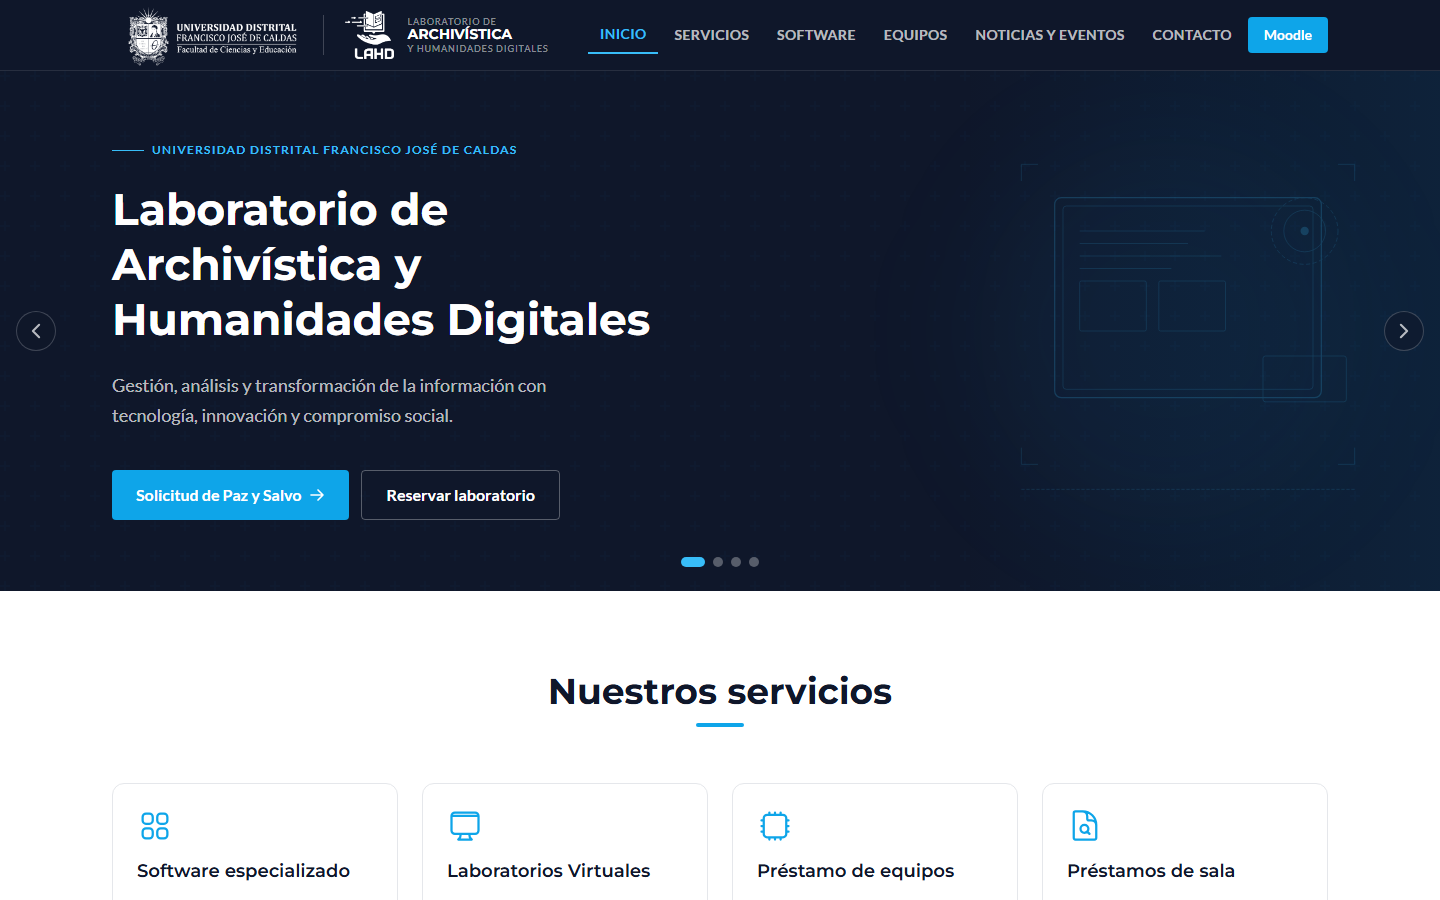
\includegraphics[width=0.92\textwidth]{capturas/portada.png}
  \caption{Página de inicio del portal del laboratorio.}
\end{figure}

\chapter{Navegación por el portal}

\section{Página de inicio}

La página de inicio está organizada en las siguientes secciones:

\begin{enumerate}
  \item \textbf{Carrusel principal} (Hero): muestra un mensaje institucional y
        rota automáticamente las 3 noticias más recientes. Puede navegar
        manualmente con las flechas \texttt{Anterior}/\texttt{Siguiente} o los
        puntos indicadores. Cada diapositiva incluye botones de acción:
        \textbf{Solicitud de Paz y Salvo} y \textbf{Reservar laboratorio}.
  \item \textbf{Servicios}: cuatro tarjetas que enlazan a las secciones
        principales: Software especializado, Laboratorios Virtuales, Préstamo
        de equipos y Préstamos de sala.
  \item \textbf{Noticias destacadas}: muestra las 4 noticias más recientes con
        imagen, fecha, autor y extracto. Incluye enlace \textbf{Ver todas} al
        listado completo.
  \item \textbf{Acceso rápido a software}: botones directos a DSpace,
        Archivematica y AtoM.
  \item \textbf{¿Cómo usar el laboratorio?}: proceso de 4 pasos (Solicitud,
        Validación, Uso del servicio, Entrega).
  \item \textbf{Contacto}: información de ubicación, correo, horario y
        descripción del proyecto curricular.
\end{enumerate}

\begin{figure}[H]
  \centering
  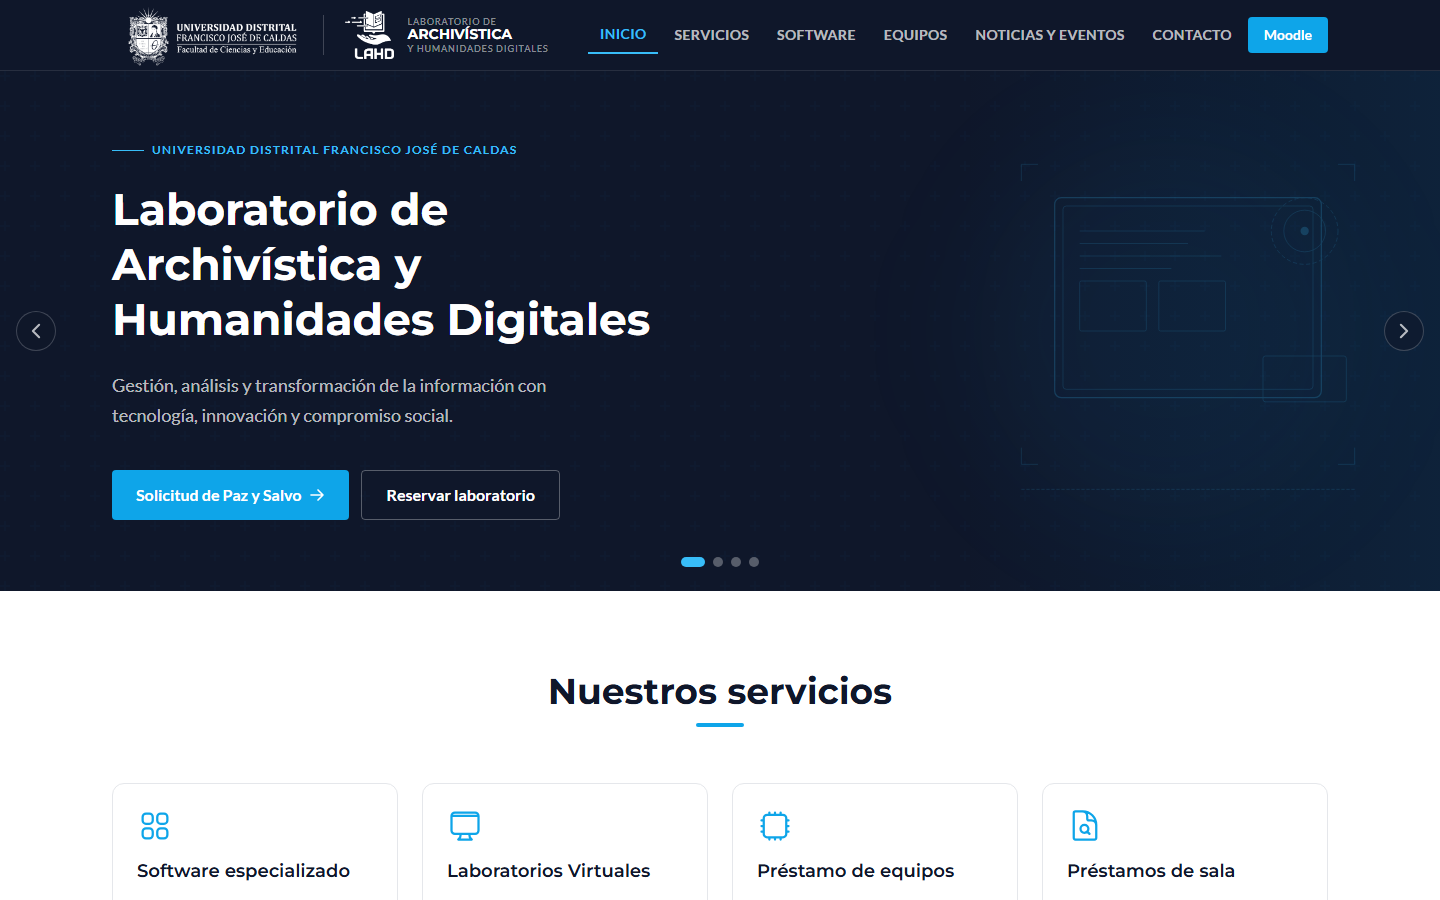
\includegraphics[width=0.92\textwidth]{capturas/portada.png}
  \caption{Página de inicio: carrusel, servicios y noticias.}
\end{figure}

\section{Sección Equipos}

La sección \textbf{Equipos} (\texttt{/equipos}) presenta el catálogo completo
de equipos disponibles para préstamo.

\begin{itemize}
  \item \textbf{Filtros}: botones \textbf{Todos} y \textbf{Disponibles} para
        filtrar el listado.
  \item \textbf{Tarjetas de equipo}: cada tarjeta muestra el nombre, una
        ilustración, descripción breve y un indicador de estado
        (\textbf{Disponible} / \textbf{No disponible}).
  \item \textbf{Enlace a detalle}: si el equipo está disponible, un botón
        \textbf{Solicitar préstamo} lleva a su ficha de detalle.
\end{itemize}

\begin{figure}[H]
  \centering
  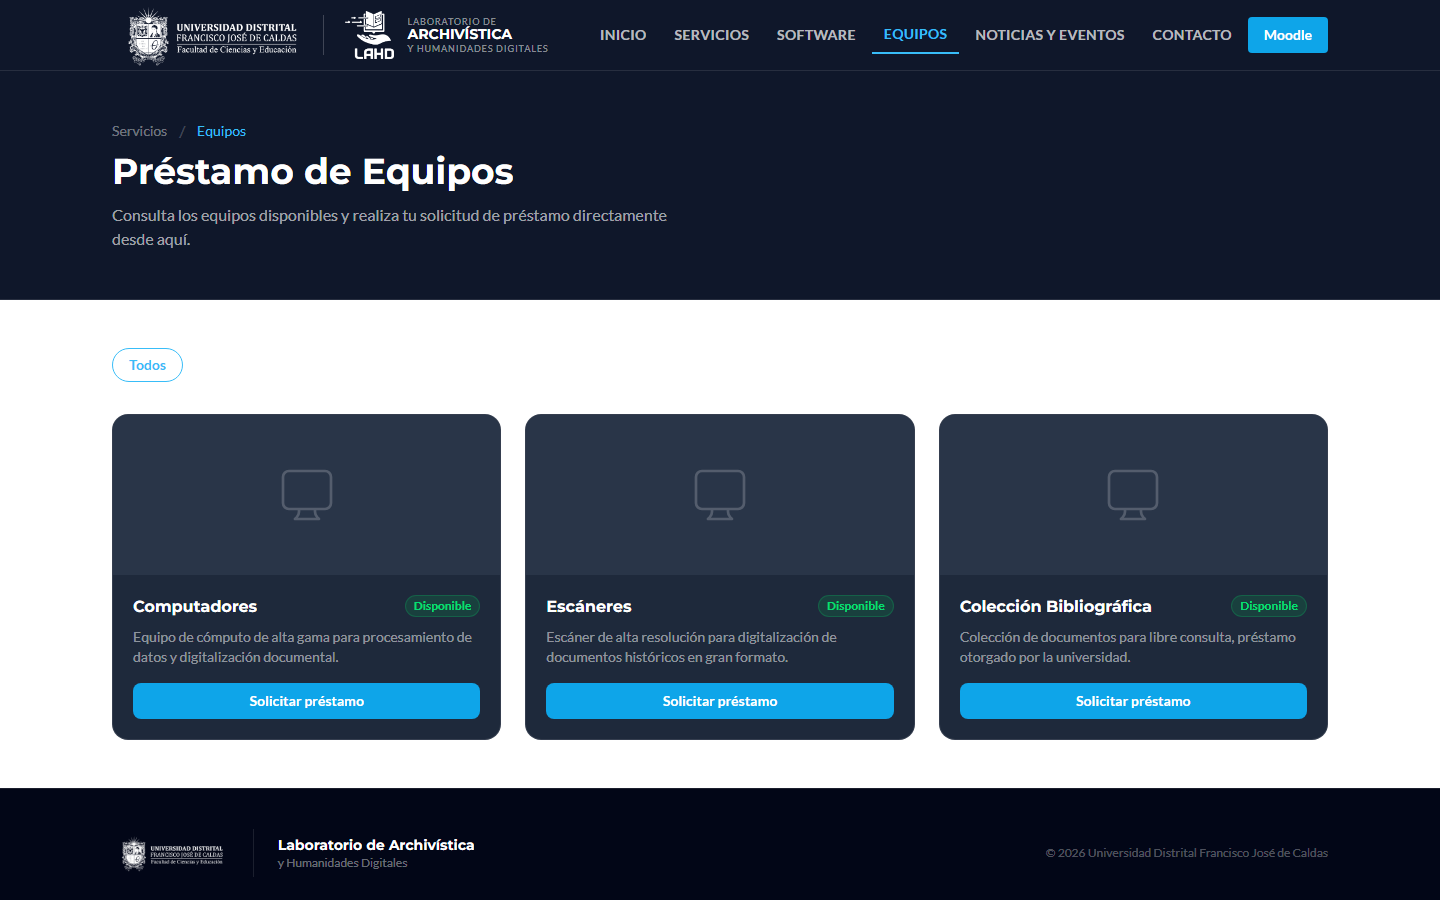
\includegraphics[width=0.92\textwidth]{capturas/equipos.png}
  \caption{Catálogo de equipos con filtros.}
\end{figure}

\subsection{Ficha de detalle de un equipo}

Al hacer clic en \textbf{Solicitar préstamo} o en la tarjeta, se abre la
página de detalle (\texttt{/equipos/<id>}) que incluye:

\begin{itemize}
  \item Nombre del equipo e indicador de disponibilidad.
  \item Descripción completa.
  \item Categoría.
  \item Botón \textbf{Solicitar por correo} (abre el cliente de correo
        institucional) si está disponible, o mensaje de no disponible.
  \item Enlace \textbf{Volver a equipos}.
\end{itemize}

\begin{figure}[H]
  \centering
  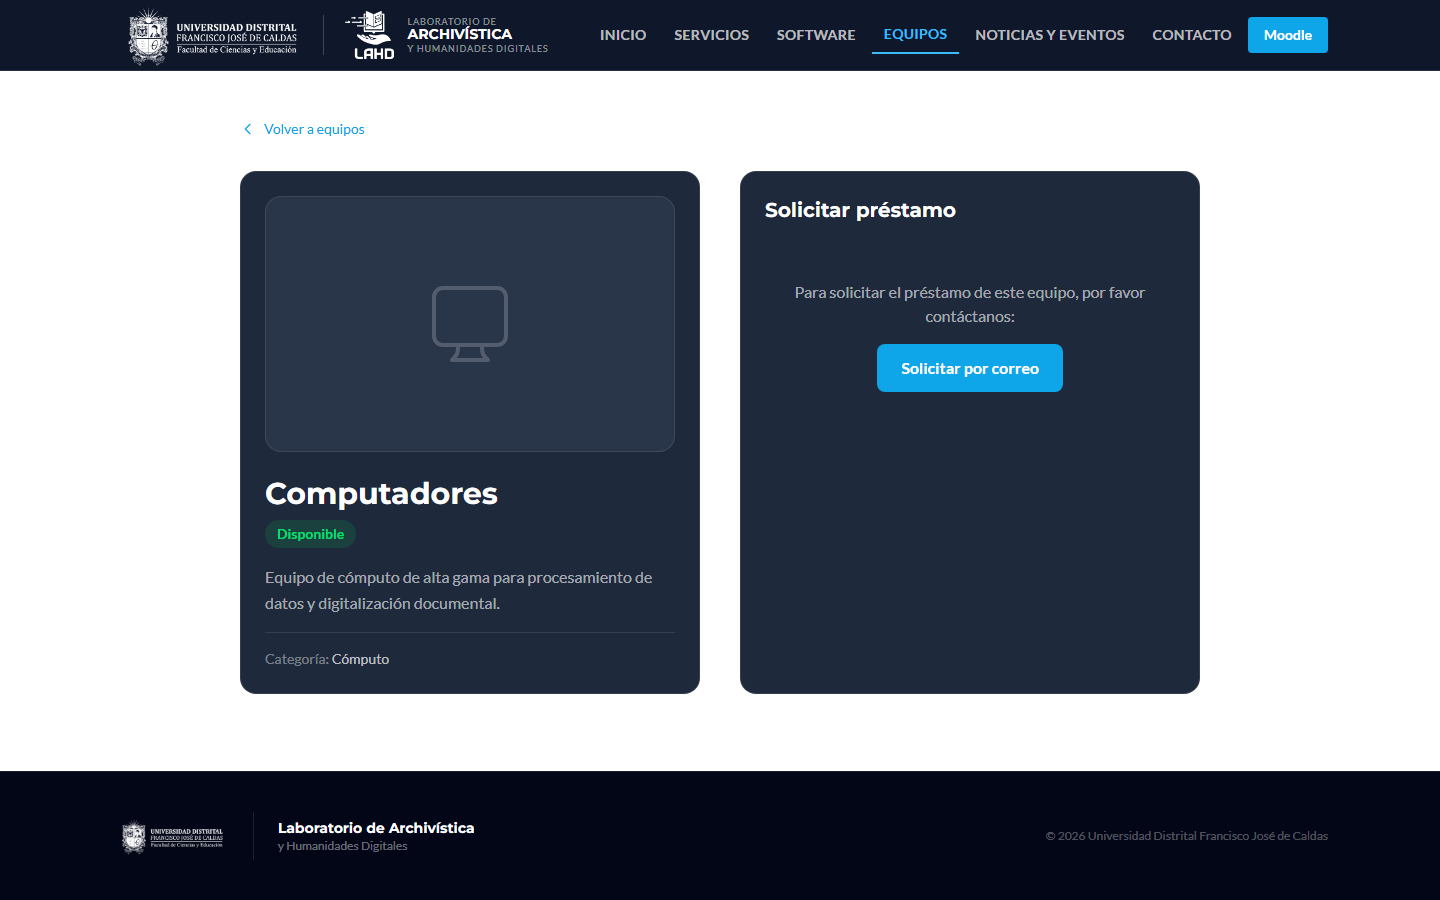
\includegraphics[width=0.92\textwidth]{capturas/equipo.png}
  \caption{Ficha de detalle de un equipo.}
\end{figure}

Los equipos disponibles en el portal son:

\begin{itemize}
  \item \textbf{Computadores} (ID 1, categoría Cómputo): equipos de cómputo de
        alta gama para procesamiento de datos y digitalización documental.
  \item \textbf{Escáneres} (ID 2, categoría Digitalización): escáner de alta
        resolución para digitalización de documentos históricos en gran formato.
  \item \textbf{Colección Bibliográfica} (ID 3, categoría Digitalización):
        documentos para libre consulta, con préstamo otorgado por la
        universidad.
\end{itemize}

\begin{mdframed}[style=importantstyle]
  \textbf{Recomendación:} revise siempre la página de detalle del equipo para
  confirmar su disponibilidad actual antes de realizar una solicitud.
\end{mdframed}

\section{Sección Software}

La sección \textbf{Software} (\texttt{/software}) reúne el catálogo de
herramientas de gestión y preservación documental disponibles en el laboratorio.

\begin{itemize}
  \item \textbf{Acceso rápido}: botones directos a DSpace, Archivematica y
        AtoM en la parte superior.
  \item \textbf{Búsqueda y filtrado}: campo de texto para buscar por nombre y
        selector de categoría.
  \item \textbf{Tarjetas de software}: cada una muestra el nombre, versión,
        categoría, tipo de licencia, descripción y, si tiene URL, un botón
        \textbf{Acceder}.
\end{itemize}

\begin{figure}[H]
  \centering
  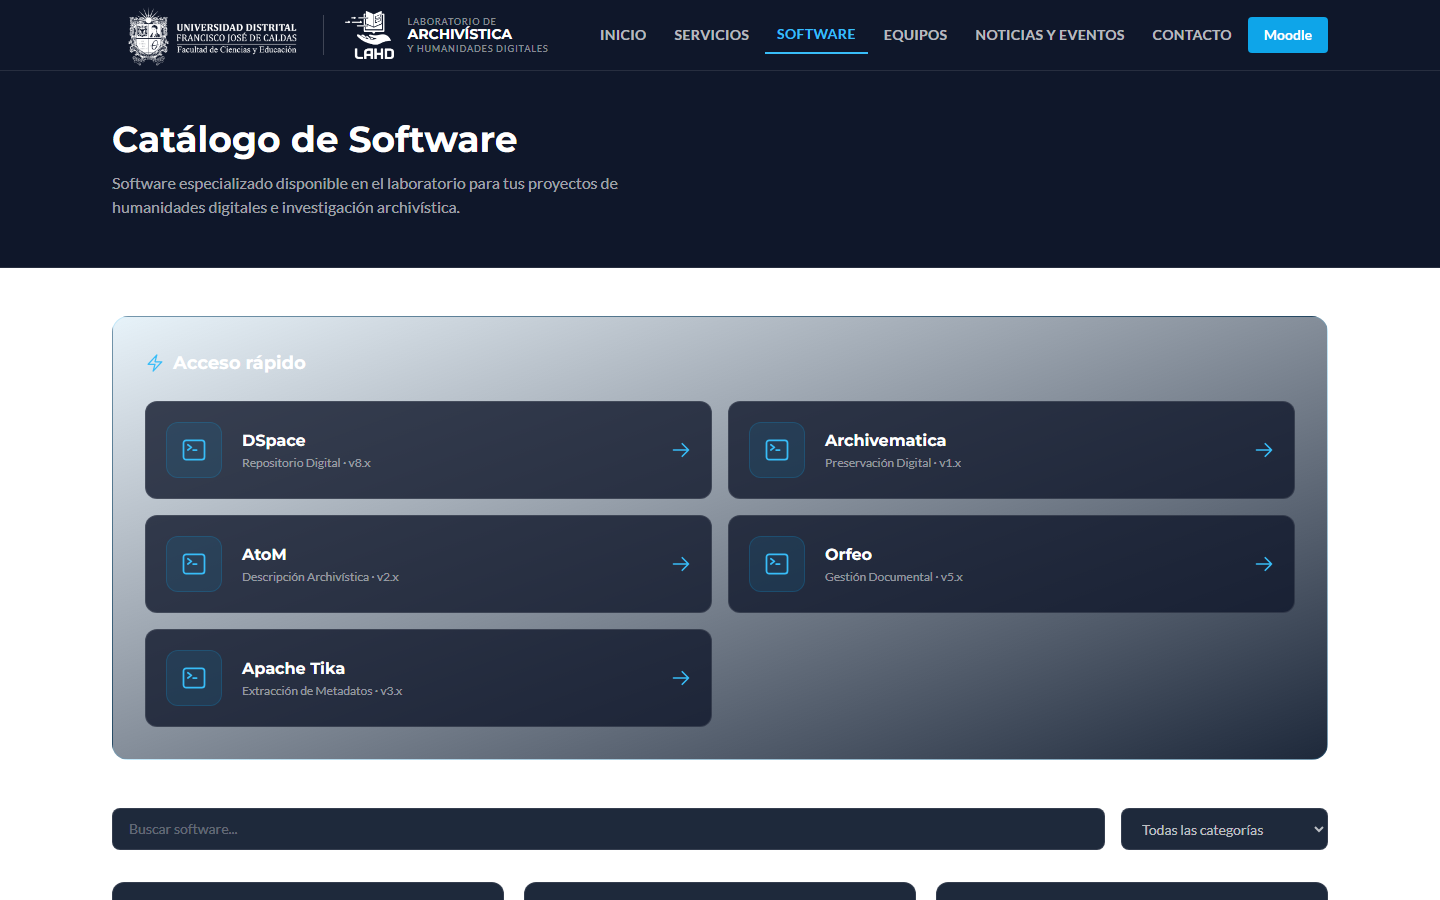
\includegraphics[width=0.92\textwidth]{capturas/software.png}
  \caption{Catálogo de software con búsqueda y filtros.}
\end{figure}

El software disponible incluye:

\begin{itemize}
  \item \textbf{DSpace} (v8.x, Repositorio Digital, Open Source): repositorio
        digital institucional para gestión, preservación y difusión de la
        producción académica. Acceso: \texttt{/dspace/}.
  \item \textbf{Archivematica} (v1.x, Preservación Digital, Open Source):
        preservación digital automatizada según OAIS, PREMIS y METS. Acceso:
        \texttt{/archivematica/}.
  \item \textbf{AtoM} (v2.x, Descripción Archivística, Open Source):
        aplicación web para descripción archivística con estándares ISAD(G),
        ISAAR(CPF) e ISDIAH. Acceso: \texttt{:63001}.
  \item \textbf{Orfeo} (v5.x, Gestión Documental, Open Source): SGDEA que
        cumple normatividad colombiana AGN y estándar MOREQ. Acceso:
        \texttt{/orfeo/}.
  \item \textbf{Apache Tika} (v3.x, Extracción de Metadatos, Apache 2.0):
        detección y extracción de metadatos y contenido en múltiples formatos.
        Acceso: \texttt{/tika/}.
  \item \textbf{ExifTool} (v13.x, Metadatos, Perl): herramienta CLI para leer,
        escribir y editar metadatos de archivos multimedia y documentos. No
        tiene interfaz web.
\end{itemize}

\section{Sección Servicios y Salas}

La sección \textbf{Servicios} (\texttt{/servicios}) presenta una vista general
de los tres servicios principales con enlaces directos, seguida de una sección
de información práctica y el proceso de solicitud de 4 pasos.

La subsección \textbf{Salas} (\texttt{/servicios/salas}) lista los espacios
disponibles para reserva:

\begin{figure}[H]
  \centering
  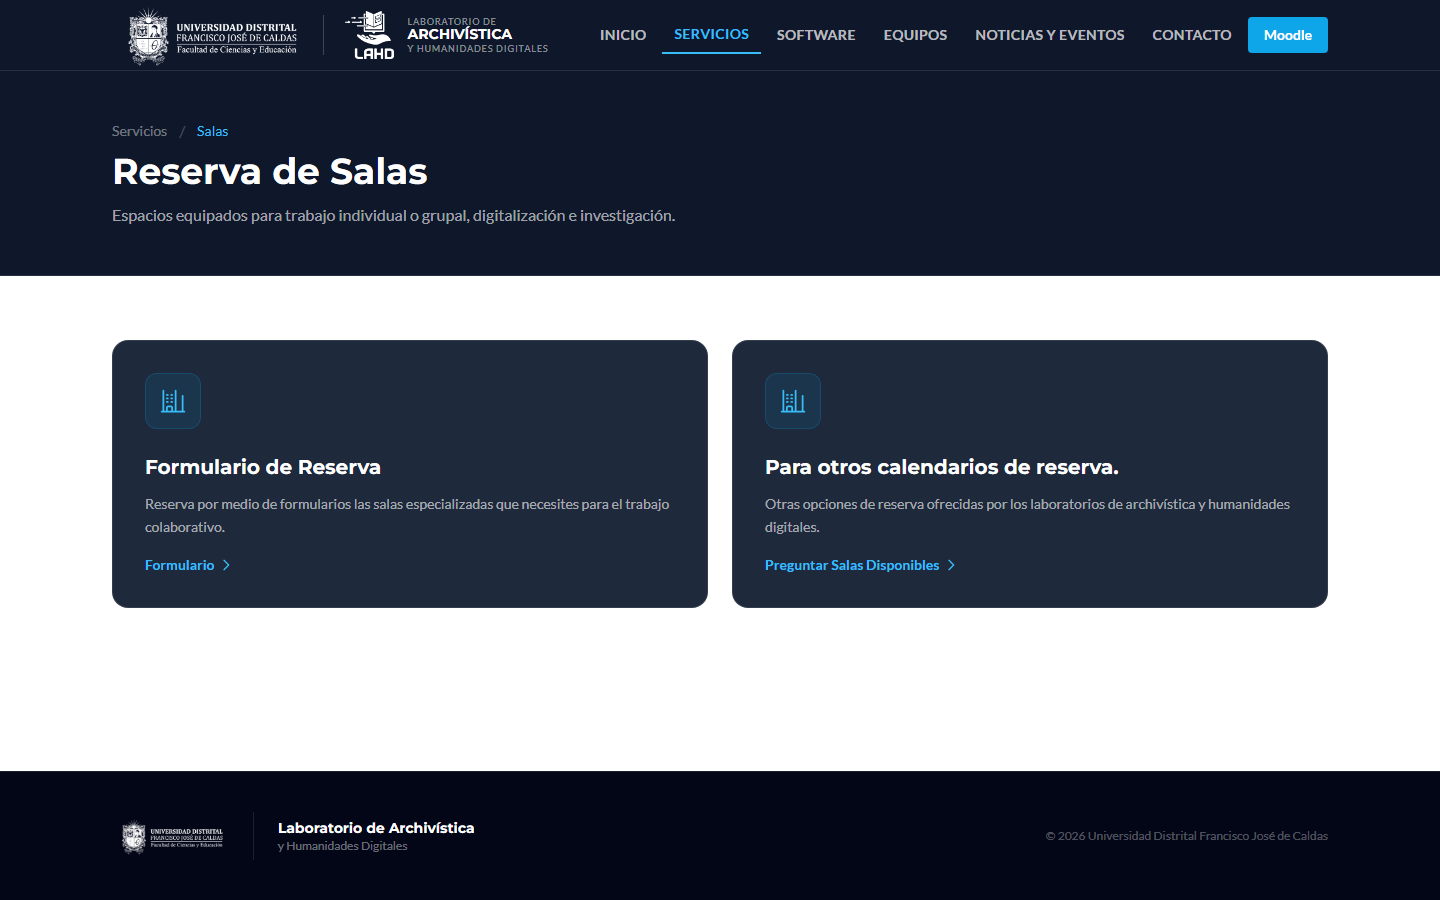
\includegraphics[width=0.92\textwidth]{capturas/salas.png}
  \caption{Listado de salas disponibles para reserva.}
\end{figure}

\begin{itemize}
  \item \textbf{Sala de Digitalización} (capacidad 6): escáneres planetarios y
        de alta velocidad para digitalización documental. Disponible.
  \item \textbf{Sala de Trabajo Colaborativo} (capacidad 12): equipos de
        cómputo y pizarra digital para trabajo en grupo. Disponible.
  \item \textbf{Cubículo de Estudio} (capacidad 2): espacio privado para
        investigación y análisis de documentos. No disponible actualmente.
\end{itemize}

Al hacer clic en una sala, se abre su ficha de detalle (\texttt{/servicios/salas/<id>})
con capacidad, descripción y un formulario de reserva.

\section{Sección Noticias}

La sección \textbf{Noticias} (\texttt{/noticias}) muestra el listado completo
de noticias en tarjetas con imagen, fecha, autor y extracto.

\begin{figure}[H]
  \centering
  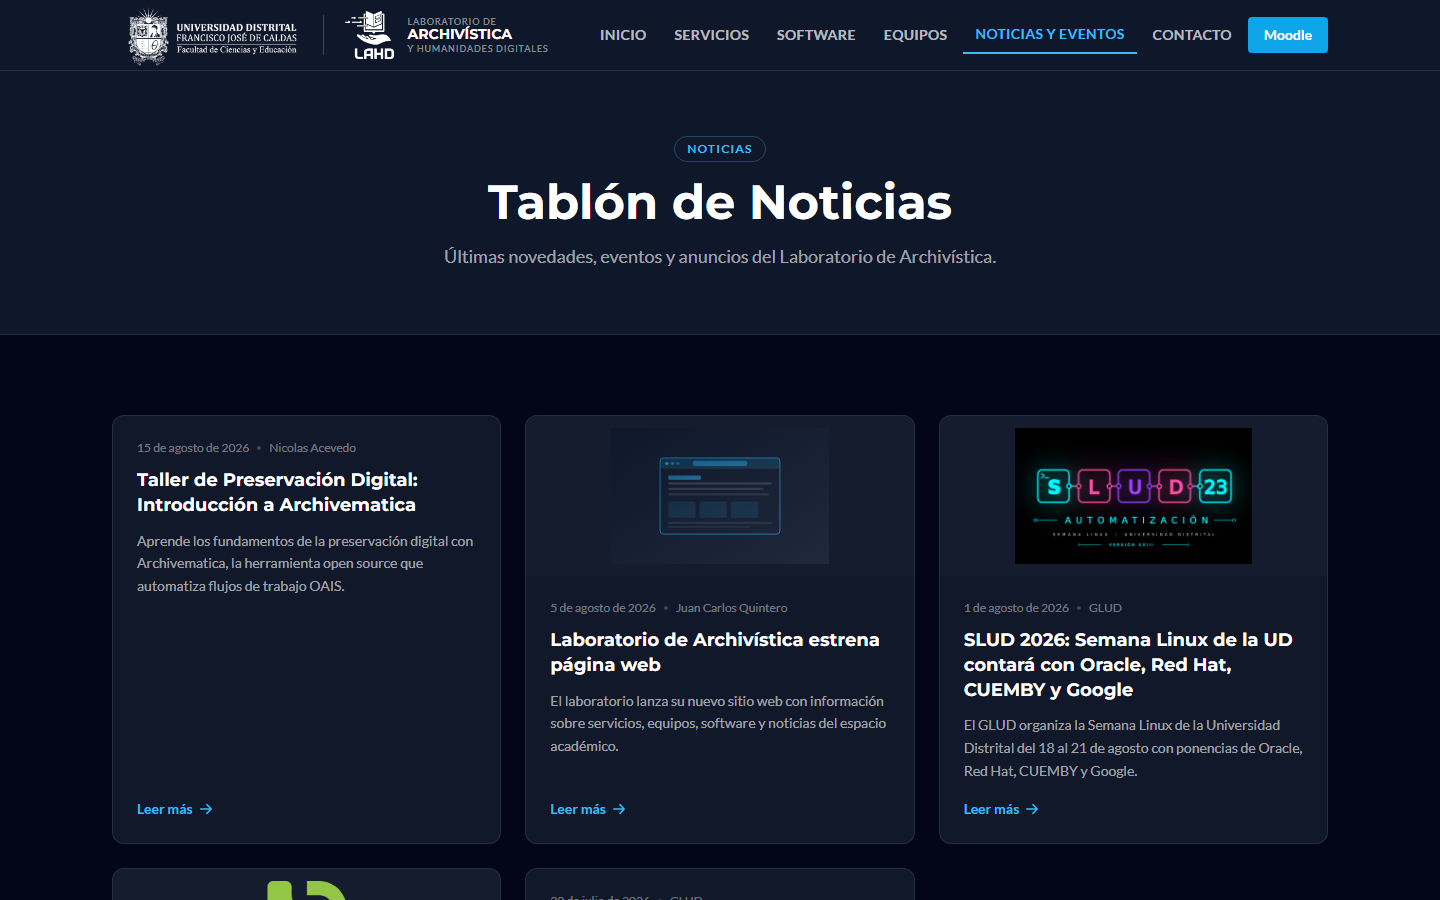
\includegraphics[width=0.92\textwidth]{capturas/noticias.png}
  \caption{Listado de noticias del laboratorio.}
\end{figure}

Para leer una noticia completa, haga clic en la tarjeta o en \textbf{Leer más}.
La página de detalle (\texttt{/noticias/<slug>}) muestra:

\begin{figure}[H]
  \centering
  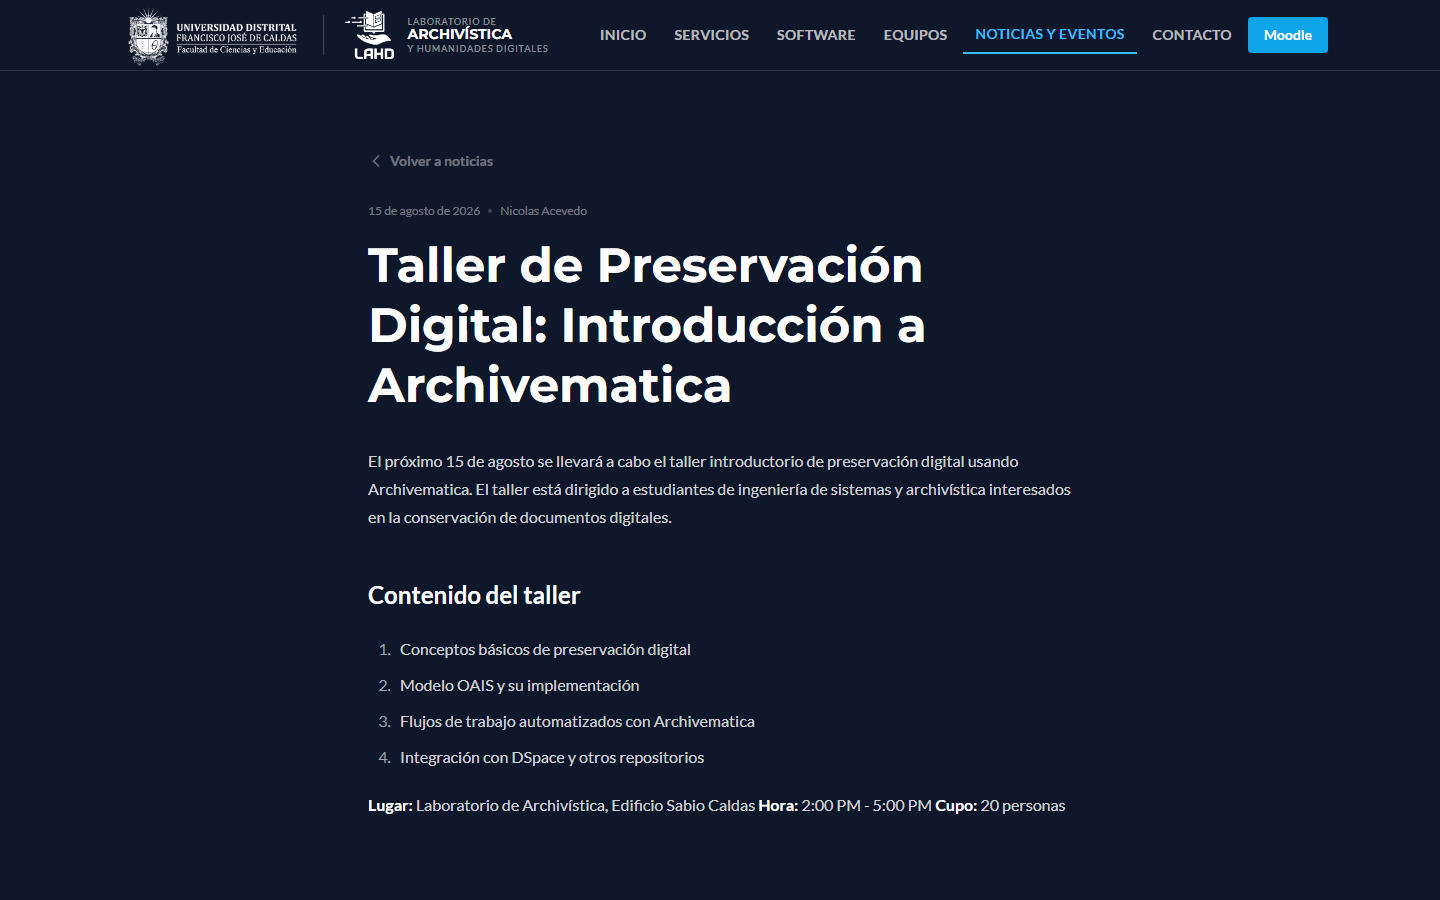
\includegraphics[width=0.92\textwidth]{capturas/noticia.png}
  \caption{Página de detalle de una noticia.}
\end{figure}

\begin{itemize}
  \item Título, fecha formateada y autor.
  \item Imagen destacada (si la tiene).
  \item Contenido completo en formato Markdown renderizado (párrafos,
        listas, enlaces, citas, etc.).
  \item Enlace \textbf{Volver a noticias}.
\end{itemize}

\section{Sección Investigación}

La sección \textbf{Investigación} (\texttt{/investigacion}) presenta los
proyectos y líneas de trabajo del laboratorio:

\begin{itemize}
  \item \textbf{Digitalización del Patrimonio}: proyectos de preservación y
        digitalización de documentos históricos y archivos universitarios.
  \item \textbf{Análisis de Datos Históricos}: aplicación de técnicas
        computacionales para análisis y visualización de datos en humanidades.
  \item \textbf{Archivística Computacional}: desarrollo de metodologías para
        la gestión automatizada de archivos digitales.
  \item \textbf{Preservación Digital}: estudio de estándares y estrategias para
        la preservación a largo plazo de documentos digitales.
\end{itemize}

\begin{figure}[H]
  \centering
  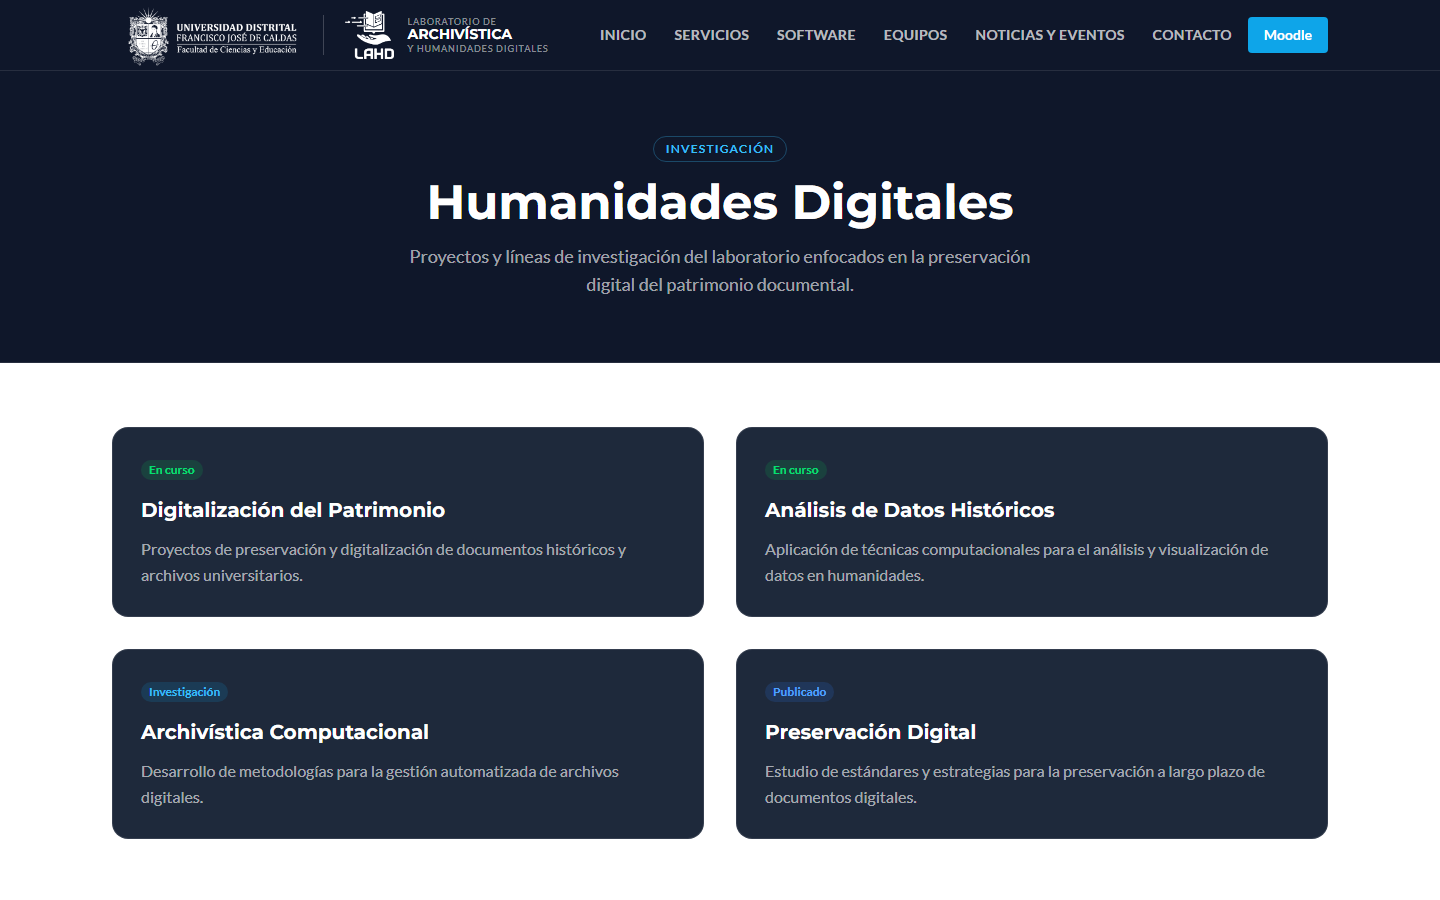
\includegraphics[width=0.92\textwidth]{capturas/investigacion.png}
  \caption{Sección de proyectos de investigación.}
\end{figure}

\chapter{Solicitud de equipos y salas}

El proceso para solicitar equipos y reservar salas sigue los cuatro pasos
mostrados en la página de inicio:

\begin{enumerate}
  \item \textbf{Solicitud}: diligencie el formulario de reserva del espacio o
        el préstamo del equipo.
  \item \textbf{Validación}: el equipo del laboratorio revisa y confirma la
        solicitud a través del correo electrónico.
  \item \textbf{Uso del servicio}: acceda al laboratorio y utilice los recursos
        asignados.
  \item \textbf{Entrega}: entregue los recursos asignados y firme el control de
        préstamos de la sala.
\end{enumerate}

\section{Préstamo de equipos}

\begin{enumerate}
  \item Ingrese a la sección \textbf{Equipos} del portal.
  \item Use los filtros \textbf{Todos} / \textbf{Disponibles} si lo desea.
  \item Seleccione el equipo que necesita y revise su ficha de detalle.
  \item Si está disponible, haga clic en \textbf{Solicitar préstamo} o contacte
        directamente al equipo del laboratorio por el correo institucional
        (\texttt{labarchivistica@udistrital.edu.co}) indicando:
        \begin{itemize}
          \item Su nombre completo y número de documento/carné.
          \item Equipo solicitado.
          \item Fecha y hora previstas de uso.
          \item Justificación breve del uso.
        \end{itemize}
  \item Espere la confirmación por correo electrónico del equipo del
        laboratorio.
  \item Reclame el equipo en las instalaciones en la fecha acordada y firme el
        control de préstamos.
\end{enumerate}

\begin{mdframed}[style=importantstyle]
  \textbf{Nota:} el préstamo está sujeto a disponibilidad y a la aprobación
  del equipo del laboratorio. El incumplimiento en la devolución puede generar
  restricciones de acceso futuro.
\end{mdframed}

\section{Reserva de salas}

\begin{enumerate}
  \item Ingrese a la sección \textbf{Servicios / Salas}.
  \item Haga clic en \textbf{Ver salas} o vaya directamente a
        \texttt{/servicios/salas}.
  \item Elija la sala según su capacidad, disponibilidad y equipamiento.
  \item Haga clic en la sala para ver su ficha de detalle.
  \item Complete el formulario de reserva (enlace externo) con:
        \begin{itemize}
          \item Datos personales (nombre, documento, correo, programa).
          \item Sala solicitada.
          \item Fecha, hora de inicio y hora de fin.
          \item Propósito de la reserva (trabajo grupal, digitalización,
                investigación individual, etc.).
        \end{itemize}
  \item Espere la confirmación por correo electrónico.
  \item Preséntese en el laboratorio a la hora acordada y firme el control de
        reserva.
\end{enumerate}

\begin{mdframed}[style=importantstyle]
  \textbf{Importante:} la reserva de salas se gestiona mediante formularios
  externos (Microsoft Forms / Microsoft Cloud Forms). Asegúrese de usar su
  correo institucional para diligenciarlos.
\end{mdframed}

\chapter{Uso de los servicios de software}

El laboratorio ofrece varias aplicaciones web de código abierto accesibles
desde el portal. La mayoría se sirven a través del proxy nginx y no requieren
instalación local.

\section{Acceso a las herramientas principales}

\begin{itemize}
  \item \textbf{DSpace} (repositorio digital):
        \url{http://labhumanidades.udistrital.edu.co/dspace/}
  \item \textbf{Orfeo} (gestión documental - UI clásica):
        \url{http://labhumanidades.udistrital.edu.co/orfeo/}
  \item \textbf{Orfeo NG} (UI moderna):
        \url{http://labhumanidades.udistrital.edu.co/orfeo-ng/}
  \item \textbf{Apache Tika} (interfaz web):
        \url{http://labhumanidades.udistrital.edu.co/tika/}
  \item \textbf{Apache Tika API} (REST):
        \url{http://labhumanidades.udistrital.edu.co/tika/api/}
  \item \textbf{Archivematica}:
        \url{http://labhumanidades.udistrital.edu.co/archivematica/}
  \item \textbf{AtoM}:
        \url{http://labhumanidades.udistrital.edu.co:63001}
  \item \textbf{ExifTool}: herramienta de línea de comandos; no tiene interfaz
        web. Se ejecuta en el servidor donde está instalado.
\end{itemize}

\begin{mdframed}[style=importantstyle]
  \textbf{Credenciales:} para DSpace, Orfeo, Archivematica y AtoM se requiere
  una cuenta de usuario. Solicite su cuenta al equipo del laboratorio
  indicando su nombre, documento y propósito de uso.
\end{mdframed}

\section{Descripción rápida de cada herramienta}

\subsection{DSpace}
Repositorio digital institucional. Permite cargar, describir, preservar y
difundir la producción académica (artículos, tesis, datos, etc.). Basado en
el modelo OAIS. Soporta búsqueda por facetas, DOIs, licencias Creative
Commons y estadísticas de uso.

\subsection{Orfeo / Orfeo NG}
Sistema de Gestión Documental y Administración de Archivos (SGDEA). Cumple
con la normatividad del Archivo General de la Nación (AGN) y el estándar
MOREQ. Funcionalidades: radicación, clasificación, expedientes, traslados,
eliminación, consulta y certificaciones. Orfeo NG es la versión moderna con
interfaz Angular.

\subsection{Archivematica}
Sistema de preservación digital automatizado. Implementa flujos de trabajo
basados en OAIS: ingestión (SIP), almacenamiento (AIP), diseminación (DIP),
verificación de integridad (fixity), migración de formatos y metadatos
PREMIS/METS.

\subsection{AtoM}
Access to Memory: aplicación web para descripción archivística multinivel
basada en estándares internacionales ISAD(G), ISAAR(CPF) e ISDIAH. Permite
crear instrumentos de investigación, autoridades, términos de materia y
exportar EAD/EAC-CPF.

\subsection{Apache Tika}
Herramienta para detección de tipo de contenido y extracción de metadatos y
texto de documentos en cientos de formatos (PDF, Office, OpenDocument,
imágenes, audio, video, etc.). Disponible como interfaz web y API REST.

\subsection{ExifTool}
Utilidad de línea de comandos (Perl) para leer, escribir y editar metadatos
EXIF, IPTC, XMP, ICC Profile, GeoTIFF, etc. en archivos de imagen, audio,
video y documentos. No tiene interfaz gráfica; se ejecuta en el servidor.

\chapter{Preguntas frecuentes (FAQ)}

\begin{itemize}
  \item \textbf{¿Quiénes pueden usar el laboratorio?}
    Estudiantes, docentes e investigadores de la Universidad Distrital
    Francisco José de Caldas con carné vigente.
  \item \textbf{¿Cómo solicito un préstamo de equipo o una reserva de sala?}
    Mediante la sección \textbf{Equipos} o \textbf{Servicios / Salas} del
    portal y la confirmación posterior por correo electrónico.
  \item \textbf{¿El software requiere instalación en mi computador?}
    No. Todas las herramientas del laboratorio se usan desde el navegador web
    (a excepción de ExifTool, que se ejecuta en el servidor).
  \item \textbf{¿Cuánto dura el préstamo de un equipo?}
    Depende de la solicitud aprobada; la duración se confirma en el correo de
    validación. Por lo general, hasta 7 días hábiles.
  \item \textbf{¿Qué hago si no recibo la confirmación por correo?}
    Verifique la carpeta de correo no deseado (spam). Si no está ahí,
    contacte directamente al equipo del laboratorio al
    \texttt{labarchivistica@udistrital.edu.co}.
  \item \textbf{¿Puedo acceder al software desde fuera de la universidad?}
    Sí, el portal es público en
    \url{http://labhumanidades.udistrital.edu.co}. Algunas herramientas
    (Archivematica, AtoM) usan puertos específicos que deben estar
    accesibles en la red.
  \item \textbf{¿Cómo publico una noticia en el portal?}
    Las noticias son gestionadas por el equipo del laboratorio. Si tiene una
    novedad para publicar, envíela a \texttt{labarchivistica@udistrital.edu.co}
    con título, fecha, extracto, autor, imagen opcional y cuerpo en Markdown.
  \item \textbf{¿Dónde encuentro los formularios de solicitud de Paz y Salvo
        y reserva de laboratorio?}
    En el carrusel de la página de inicio, botones \textbf{Solicitud de Paz
    y Salvo} y \textbf{Reservar laboratorio} (enlaces a formularios Microsoft
    Forms).
  \item \textbf{¿El laboratorio presta equipos para uso externo (fuera de la
        sede)?}
    Generalmente no. Los equipos se usan dentro de las instalaciones del
    laboratorio. Consulte casos excepcionales con el equipo.
\end{itemize}

\chapter{Contacto y soporte}

Para dudas, sugerencias, solicitudes de préstamo, reserva de salas, cuentas de
software o reporte de incidencias, contacte al equipo del Laboratorio de
Archivística y Humanidades Digitales:

\begin{itemize}
  \item \textbf{Institución}: Universidad Distrital Francisco José de Caldas,
        Facultad de Ingeniería, Proyecto Curricular de Archivística y Gestión
        de la Información Digital.
  \item \textbf{Portal web}: \url{http://labhumanidades.udistrital.edu.co}
  \item \textbf{Correo electrónico}:
        \texttt{labarchivistica@udistrital.edu.co}
  \item \textbf{Ubicación física}: Sede Ciudadela Universitaria Bosa Porvenir,
        Bloque 3, Piso 4, Sala 407, Bogotá, Colombia.
  \item \textbf{Horario de atención}: Lunes a Viernes, 8:00 a.m. -- 4:00 p.m.
\end{itemize}

\begin{mdframed}[style=importantstyle]
  \textbf{Reporte de incidencias técnicas:} al contactar al equipo por una
  falla del portal, incluya: (1) URL donde ocurre el problema, (2) pasos
  para reproducirlo, (3) navegador y versión, (4) captura de pantalla si
  es posible, (5) fecha y hora.
\end{mdframed}

\end{document}
